\section{Implementation}\label{sec:02_impl}
% What
This section describes the most important parts of the implementation of the application.
% What technology


\subsection{Database Routine}
% Intro
A database routine needs to be implemented to seed the database, that is supposed to be used in the application.
% No EJB
This routine is not implemented as a EJB, instead, it will run as a standalone Java application.
% What data
The accommodations, as well as the occupancies of accommodatios are given by the task description.

% Technology
The following technologies are used to implement the database routine:
\begin{itemize}
\item Hibernate
\item JPA
\end{itemize}

\subsubsection{Entities}
% What
\Fig{fig:subsubsec:02_impl_db_entities} visualizes the UML diagram of the entities, used for the database.
% Overall
Overall, the database is used to save the following information:
\begin{itemize}
\item Accommodations which represent either an apartment or a hotel
\item Occupancy, represents the availability of an accommodation entity for a specific day
\item Reservation which represent a single reservation made by a user
\end{itemize}

% Figure
\begin{figure}[h]
\centering
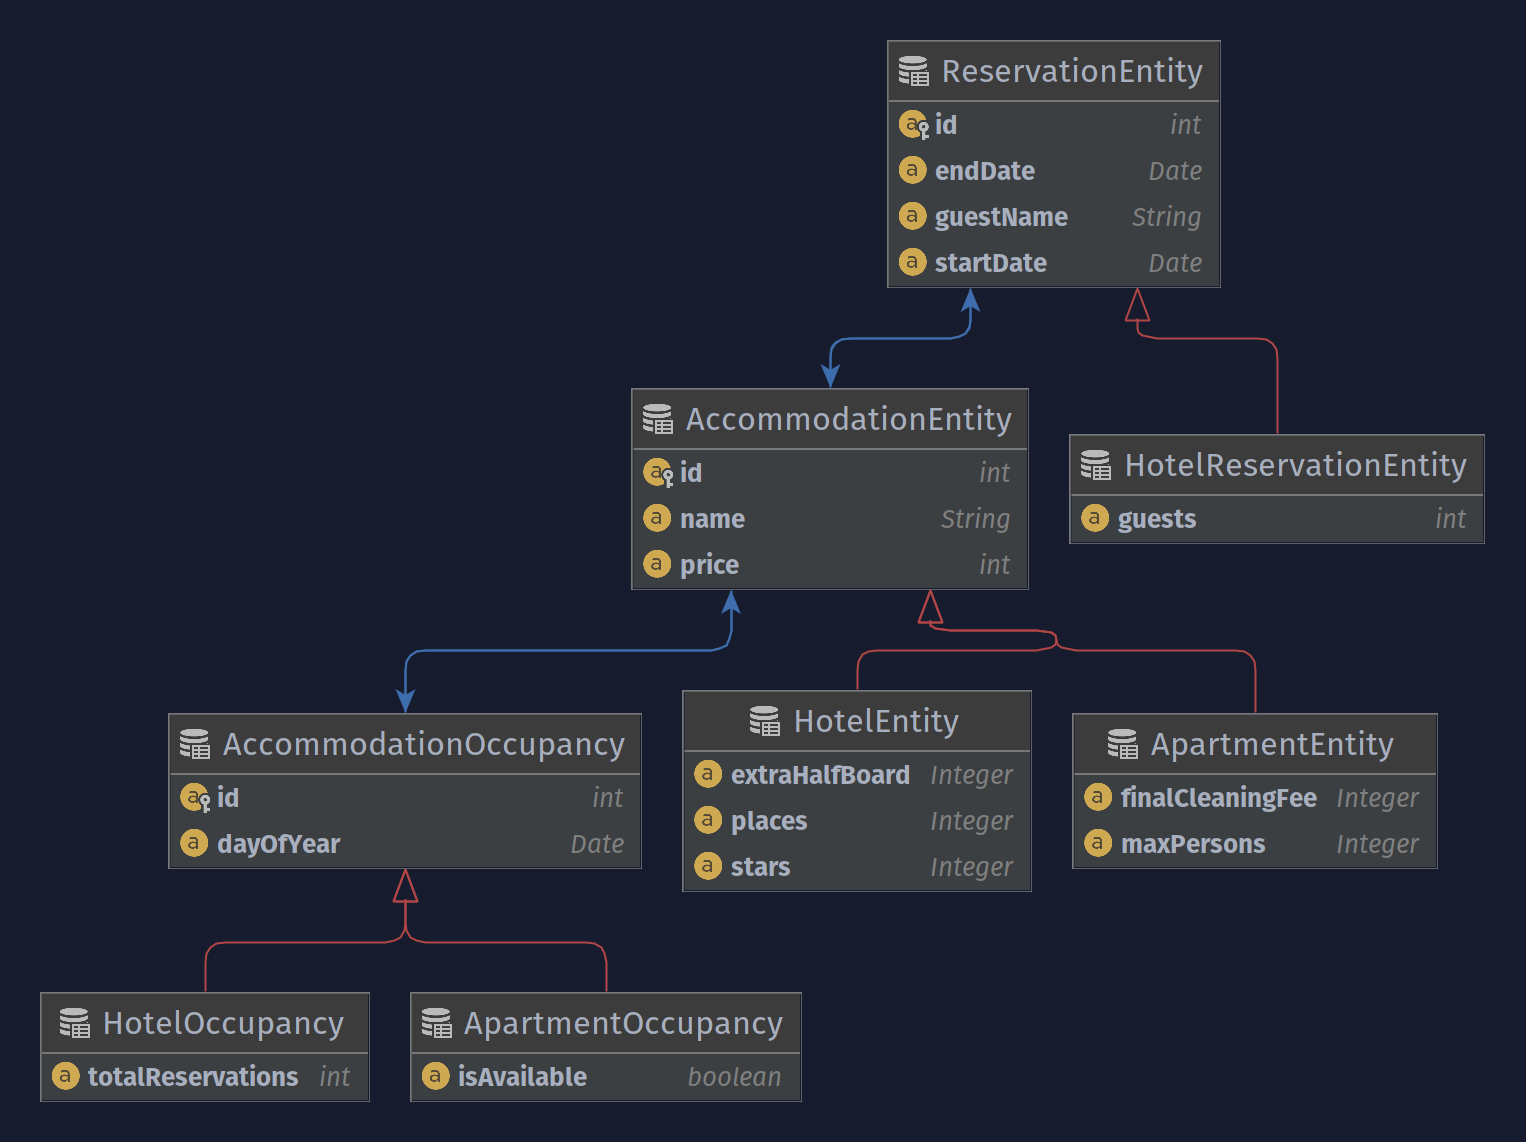
\includegraphics[scale=0.3]{images/02_impl/entities}
\caption{UML diagram of all database entities}
\label{fig:subsubsec:02_impl_db_entities}
\end{figure}

% Accommodatins
\paragraph{Accommodations}
Two types of accommodations exists for this application: Apartments and Hotels. 
% Properties
All accommadtions have a name, and a daily price. Additionally, an apartment has a final cleaning fee, an a number of maximum persons. A hotel has a rating of start, a number of free places, and a price for extra half-board.

% Classes
To implement the entities, an ApartmentEntity, and a HotelEntity have been implemented. Both classes inherit from the abstract AccommodationEntity class.


% Occupancies
\paragraph{Occupancies}
% What
Each accommodation needs an occupancy information for a specific date. The occupancy information describes if an accommodation is available on a specific date. The difference between an apartment and a hotel is, that a hotel has a specific number of reservation, and an aprtment is either available or unavaible, independetly of the number of persons.

% classes
To implement the occupancies, a parent class called HotelOccupancy exists, that includes only the date. Additionally, a class called ApartmentOccupancy saves the occupancies information for a hotel, which includes a boolean value called isAvailable that specifies, if the aprtment is avaiable for the specific date or not. Furthemore, a class called HotelEntity represent the occupancy of a hotel, which is a number of reservation for a specific date.


% Reservations
\paragraph{Reservations}
% What 
A user can make reservation that are saved to the database. A reservation consists of a start date and an end date that represent the date interval of the stay, and the name of the guest. These informations are saved by the ReservationEntity. Additionally, a classes called HotelReservationEntity, which inherits the ReservationEntity, is used to save the number of guests for on reservation of a hotel. An apartment does not need extra information, because it is either avaible or not, which is represented by the existance of a ReservationEntity in the table for the specific apartment for a specific date interval.




\subsection{Enterprise Java Beans}

\subsection{Web Application}



\subsection{Loading and caching Data}\label{subsec:02_impl_data}
% What
To be able to present all members of the Scottish parliament with all their detailed information, the application needs to load the following data:
\begin{itemize}
\item Members - Representing a member of the Scottish parliament
\item Parties - Representing a party of the Scottish parliament
\item Member-Parties - Representing a relation between a member and a party
\item Websites - Representing a website, associated with a member
\end{itemize}


\subsubsection{Loading single Data Objects}\label{subsubsec:02_impl_data_loading}
An API URL exists for each data, that presents the data in JSON format. To load the data, a service is created for each data mentioned previously.

\Lst{lst:02_impl_data_memberservice} shows the implementation of the \texttt{MemberService} to load the Member JSON data.
% The listing
\begin{lstlisting}[label=lst:02_impl_data_memberservice, caption=\texttt{MemberService} implementation, language=java]
export class MemberService {

  private readonly membersApiUrl: string = 'https://data.parliament.scot/api/members';

  constructor(private http: HttpClient) { }

  public fetchData(): Observable<Member[]> {
    return this.http
      .get<MemberResponse[]>(this.membersApiUrl)
      .pipe(
        map(response => response.map(memberResponse => new Member(memberResponse)))
      );
  }
}
\end{lstlisting}

% Describe more
First, the \texttt{MemberService} loads all members from a given URL. Then, it maps each entry of the response to a model.
% Routine for all
This routine is used for each service that loads data from the previously mentioned list.


\subsubsection{Loading all Data at once}\label{subsubsec:02_impl_data_loadingAll}
% WHat
To make the application run smoothly, it is important to load all data when the user starts the application (visits the application via a web browser).
% Intro dataservice
For this purpose, the \texttt{DataCacheService} has been implemented. It is responsible to load all previously mentioned data, by using their corresponding service. After that, it stores the data in \texttt{Observables}. This caching routine is important because otherwise all data will be loaded each time the user makes a request to the application.
% Interaction with components
After that, components can access the needed data models through these \texttt{Observables}.


% How
\Lst{lst:02_impl_data_dataserviceloading} shows a part of the implementation of the \texttt{DataCacheService}. It uses the \texttt{forkJoin} method on all data services to load and join all data at once. After the data is loaded, it saves the models (generated by the associated service) in an \texttt{Observable}.
% Already load
To check if the data has already been loaded previously, it uses the \texttt{isDataAlreadyFetched} method, which checks if the \texttt{Observables} are undefined or not.
% The listing
\begin{lstlisting}[label=lst:02_impl_data_dataserviceloading, caption=Implementation of fetching all data at once, language=java]
if (!this.isDataAlreadyFetched()) {
  let requestSources: DataRequestSources = {
    members: this.memberService.fetchData(),
    memberParties: this.memberPartyService.fetchData(),
    parties: this.partyService.fetchData(),
    websites: this.websiteService.fetchData()
  };

  let promise = new Promise<DataResponse>((resolve, reject) =>
    forkJoin(requestSources)
    .subscribe(responses => {
      this.members$ = from(responses.members);
      this.memberParties$ = from(responses.memberParties);
      this.parties$ = from(responses.parties);
      this.websites$ = from(responses.websites);

      resolve({
        members$: this.members$,
        memberParties$: this.memberParties$,
        parties$: this.parties$,
        websites$: this.websites$
      })
    }, error => {
      reject(error);
    })
  );
}
\end{lstlisting}


\newpage
\subsection{Member List}\label{subsec:02_impl_memberlist}
% Intro
The \texttt{MemberListComponent} presents all members in a grid.


% How
\Lst{lst:02_impl_memberlist_ngoninit} shows the implementation of the \texttt{ngOnInit} method of the \newline \texttt{MemberListComponent}. It uses the \texttt{fetchData} method of the \texttt{DataCacheService} to load all data (if not loaded previously, introduced in \Sec{subsubsec:02_impl_data_loadingAll}). Then, it subscribes to the \texttt{members\$} \texttt{Observable} of the \texttt{DataCacheService} to add each member to a grid property (2-dimensional array).
% Explain template
This grid property is used to build the grid in the component's template, which is shown in \Lst{lst:02_impl_memberlist_template}.

\begin{lstlisting}[label=lst:02_impl_memberlist_ngoninit, caption=\texttt{MemberListComponent} \texttt{ngOnInit} implementation, language=java]
ngOnInit(): void {
  this.dataCacheService
  .fetchData()
  .then(dataResponse =>
    dataResponse.members$.subscribe(member => this.addMemberToGrid(member))
  )
  .catch(error => console.log('ERROR', error));
}
\end{lstlisting}


% Template listing
\begin{lstlisting}[label=lst:02_impl_memberlist_template, caption=Template of \texttt{MemberListComponent}, language=HTML]
<div class="container">
  <div *ngFor="let row of grid" class="row member-row">
    <div *ngFor="let member of row" class="col-md-4">
      <app-member-card [member]="member"></app-member-card>
    </div>
  </div>
</div>
\end{lstlisting}


\newpage
\subsection{Detail Page}\label{subsec:02_impl_detail}
% What
The \texttt{DetailPageComponent} displays the detailed information for a selected member.
After the user clicks on a list item of the \texttt{MemberListComponent} (introduced in \Sec{subsec:02_impl_memberlist}), the user is redirected to the detail page.


% Receive id
A detail page of a member is available via the URL \path{http://localhost:8080/#/detail/MEMBER_ID}. Therefore, it is needed to parse the member id from the URL. After that, the member id is saved as an \texttt{Observable}. This is shown in \Lst{lst:02_impl_detail_receiveMemberId}.
% Receive id implementation
\begin{lstlisting}[label=lst:02_impl_detail_receiveMemberId, caption=Implementation of \texttt{receiveMemberId}, language=java]
private receiveMemberId(): void {
  this.memberId$ = this.route.paramMap.pipe(
    switchMap(params => {
      let memberId = Number(params.get('memberId'));
      return of(memberId);
    })
  );
}
\end{lstlisting}

% How
After the member id has been received, it is possible to subscribe to the \texttt{memberId\$} \texttt{Observable} to get the associated member data.
\Lst{lst:02_impl_detail_ngoninit} shows the implementation of the \texttt{ngOnInit} method of the \texttt{DetailPageComponent}. Like the \texttt{MemberListComponent}, it loads all data (if needed) using the \texttt{DataCacheService}. After that, it receives the member id and gets the data of the selected member.
% on init
\begin{lstlisting}[label=lst:02_impl_detail_ngoninit, caption=\texttt{ngOnInit} implementation of the \texttt{DetailPageComponent}, language=java]
ngOnInit(): void {
  this.receiveMemberId();

  if (typeof this.memberId$ !== 'undefined') {
    this.dataCacheService.fetchData().then(_ =>
      this.memberId$?.subscribe(memberId => {
        this.receiveMember(memberId);
        this.receiveWebsites(memberId);
        this.receiveParties(memberId);
      })
    );
  }
}
\end{lstlisting}


% get member
\Lst{lst:02_impl_detail_receivemember} shows the implementation of the \texttt{receiveMember} method. After the id has been received, it subscribes to the \texttt{members\$} property of the \texttt{DataCacheService} and uses a filter operation to get the member model for the requested member id.
% receive member
\begin{lstlisting}[label=lst:02_impl_detail_receivemember, caption=Implementation of the \texttt{receiveMember} method, language=java]
private receiveMember(memberId: number): void {
  this.dataCacheService.members$?.pipe(
    filter(member => member.id == memberId)
  ).subscribe(member => this.member = member);
}
\end{lstlisting}


% Get parties
Another important implementation is the way how parties are associated with a member. This implementation is shown in \Lst{lst:02_impl_detail_receiveParties}.
% Filter for member
At first, only the \texttt{MemberParties} objects are received that are associated with the current member using the member id.
% Group together
Then, it is needed to group \texttt{MemberParties} together, because a member can be in different parties or in the same party multiple times for different time intervals.

% Get memberships
After the \texttt{MemberParties} have been grouped, parties of the same type have to be merged together. At this point, it is important to save the smallest \textit{from} date, and the largest \textit{until} date (if defined, \textit{until} can be \texttt{null}). Then, it is possible to show the length of the membership.

% Get parties
Next, the \texttt{Party} models need to be received from the \texttt{parties\$} \texttt{Observable} of the \texttt{DataCacheService} using the \texttt{partyId} of the \texttt{MemberParty}.
% Push to array
At last, an object containing the \texttt{Party} model, and the \textit{from} and \textit{until} dates are pushed to an array. This is necessary, to list them in the \texttt{DetailPageComponent} template.
% Get Parties code
\begin{lstlisting}[label=lst:02_impl_detail_receiveParties, caption=Implementation of the \texttt{receiveParties} method, language=java]
private receiveParties(memberId: number) {
  this.dataCacheService.memberParties$?.pipe(
    filter(memberParty => memberParty.personId == memberId),
    groupBy(memberParty => memberParty.partyId),
    mergeMap(group =>
      group.pipe(
        toArray(),
        map(groupedParties => this.generateMembership(groupedParties))
      )
    )
  ).subscribe(membership => {
    this.dataCacheService.parties$?.pipe(
      filter(party => party.id == membership.memberParty.partyId),
      map(party => {
        return {party, from: membership.from, until: membership.until};
      })
    ).subscribe(partyMembership => this.partyMemberships.push(partyMembership));
  });
}
\end{lstlisting}
